%%%%%%%%%%%%%%%%%%%%%%%%%%%%%%%%%%%%%%%%%%%%%%%%%%%%%%%%%%%%%%%%%%%%%%%%%%%%%%%%
% ISE Lab -- Topic
% Giovanni Ciatto
% Alma Mater Studiorum - Università di Bologna
% mailto:giovanni.ciatto@unibo.it
%%%%%%%%%%%%%%%%%%%%%%%%%%%%%%%%%%%%%%%%%%%%%%%%%%%%%%%%%%%%%%%%%%%%%%%%%%%%%%%%
%\documentclass[handout]{beamer}\mode<handout>{\usetheme{default}}
%
\documentclass[presentation]{beamer}\mode<presentation>{\usetheme{AMSBolognaFC}}
%\documentclass[handout]{beamer}\mode<handout>{\usetheme{AMSBolognaFC}}
%%%%%%%%%%%%%%%%%%%%%%%%%%%%%%%%%%%%%%%%%%%%%%%%%%%%%%%%%%%%%%%%%%%%%%%%%%%%%%%%
\usepackage{ise-lab-common}
\usepackage{ise-lab-perception-actuation}
% version
\newcommand{\versionmajor}{0}
\newcommand{\versionminor}{1}
\newcommand{\versionpatch}{1}
\newcommand{\version}{\versionmajor.\versionminor.\versionpatch}
%%%%%%%%%%%%%%%%%%%%%%%%%%%%%%%%%%%%%%%%%%%%%%%%%%%%%%%%%%%%%%%%%%%%%%%%%%%%%%%%
\title[\currentLab{} -- Perception \& Actuation]{Perception \& Actuation from the Agent Perspective}
%
\subtitle{\courseName{} / Module \moduleN{} (\courseAcronym)}
%
\author[\sspeaker{\gcShort}]{\speaker{\gcFull} \\ \gcEmail}
%
\institute[\disiShort, \uniboShort]{\disi{} (\disiShort)\\\unibo}
%
\date[A.Y. \academicYear{} (v.\ \version)]{Academic Year \academicYear{}\\(version \version)}
%
%%%%%%%%%%%%%%%%%%%%%%%%%%%%%%%%%%%%%%%%%%%%%%%%%%%%%%%%%%%%%%%%%%%%%%%%%%%%%%%%
\begin{document}
%%%%%%%%%%%%%%%%%%%%%%%%%%%%%%%%%%%%%%%%%%%%%%%%%%%%%%%%%%%%%%%%%%%%%%%%%%%%%%%%

%/////////
\frame{\titlepage}
%/////////

%%===============================================================================
\section*{Outline}
%%===============================================================================
%
%%/////////
\frame[c]{\tableofcontents[hideallsubsections]}
%%/////////

%===============================================================================
\section{Premises}
%===============================================================================

\begin{frame}{Lecture Goals}
    \begin{itemize}
        \item Understand how to enable the perception and actuation from the agent perspective
        \item Understand the notion of layered software system
        \item Understand the key role of Application Programming Interfaces (API)
    \end{itemize}
\end{frame}

%===============================================================================
\section{(Software) Environments}
%===============================================================================

\begin{frame}{The Role of Perception and Actuation}
    \begin{block}{\textbf{Environment} = anything laying outside the \textbf{agents}}
        \begin{itemize}
            \item
              Can be \alert{perceived} via \emph{sensors}
            \item
              Can be \alert{affected} via \emph{actuators}
        \end{itemize}
    \end{block}

    \begin{center}
        \includegraphics[width=.5\linewidth]{figures/agent-environment.png}
    \end{center}

    \begin{alertblock}{About \textbf{computational} agents}
        \begin{itemize}
            \item `Perception' $\approx$ \alert{input}
            \item `Actuation' $\approx$ \alert{output}
        \end{itemize}
    \end{alertblock}
\end{frame}

\begin{frame}{Layered View of the Software Agent}
    Software agents can be abstractly modelled as composed by \alert{layers}:
    %
    \begin{columns}
        \begin{column}{.5\linewidth}
            \begin{enumerate}
                \item Some control software
                %
                \begin{itemize}
                    \item[eg] Java / logic / AgentSpeak program
                \end{itemize}
                
                \item Some interpreter for that software (e.g.~JVM, Prolog interpreter, Jason)
                %
                \begin{itemize}
                    \item[eg] Java / logic interpreter, Jason
                \end{itemize}

                \item Some OS mediating the usage of HW resources for the interpreter
                
                \item Hardware resources
                %
                \begin{itemize}
                    \item[eg] memory, storage, computational power, I/O (there including networking)
                \end{itemize}
            \end{enumerate}
        \end{column}
        \begin{column}{.5\linewidth}
            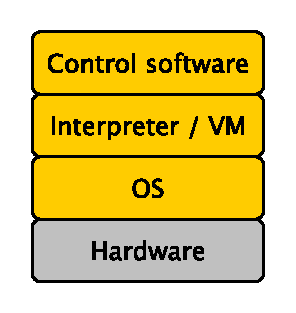
\includegraphics[width=\linewidth]{figures/layers.pdf}
        \end{column}
    \end{columns}
\end{frame}

\begin{frame}[allowframebreaks]{Actions from the Agent Perspective}
    \begin{itemize}
        \item The environment is shaped by what perceptual/actuatory actions agents can perform
        %
        \begin{itemize}
            \item[eg] sensing enviromental properties (temperature, humidity, light, etc.)
            \item[eg] sensing distances, obstacles, etc.
            \item[eg] moving wheels or harms, sucking or pushing air, etc. 
        \end{itemize}

        \vfill

        \item The agent may also be endowed with \alert{epistemic} capabilities
        %
        \begin{itemize}
            \item[eg] memorise new knowledge
            \item[eg] forget (or update) memorised knowledge
        \end{itemize}
    \end{itemize}

    \framebreak

    \begin{alertblock}{Actions may \textbf{fail} (in so many ways!)}
        \begin{itemize}
            \item[a.] perceptual actions may provide \alert{imprecise} or \alert{meaningless} percept
            %
            \begin{itemize}
                \item[b.] or fail in providing a percept at all
            \end{itemize}

            \item[c.] actuatory actions may \alert{silently} fail by \alert{provoking no effect}
            %
            \begin{itemize}
                \item[d.] or explicitly fail returning some feedback to the agent
            \end{itemize}
        \end{itemize}        
    \end{alertblock}
    %
    \begin{itemize}
        \item situations \alert{a.} and \alert{c.} are very subtle to spot
        %
        \begin{itemize}
            \item since they're undistinguishable from `correct' actions
        \end{itemize}

        \item situations \alert{b.} and \alert{d.} subtend some form of \alert{proprioception}
    \end{itemize}
\end{frame}

\begin{frame}[allowframebreaks]{Actions from the \textbf{Software} Agent Perspective}

    \begin{alertblock}{Endowing agents with some perceptual/actuatory action requires}
        \begin{enumerate}
            \item some enabling HW facility to be present
            \item some OS functionality enabling the usage of that HW facility
            \item the interpreter to know how to call that OS functionality
            \item the programming language to have some ad-hoc API wrapping the OS functionality
        \end{enumerate}
    \end{alertblock}

    \begin{exampleblock}{The file system as an environment}
        \begin{itemize}
            \item \alert{reading} a file as a string, given its path as the \alert{perception} action
            %
            \begin{itemize}
                \item fails explicitly  when the path is missing, or non-readable
            \end{itemize}

            \item \alert{writing} a file as a string, given its path as the \alert{actuation} action
            %
            \begin{itemize}
                \item fails when the path is missing, or non-readable
            \end{itemize}
        \end{itemize}
    \end{exampleblock}
\end{frame}

\section{Logic Agents}

\begin{frame}[allowframebreaks]{Prolog Agents}
    \prologimport{listings/logic-agent-stub.pl}

    \prologimport{listings/thermostat-agent.pl}
\end{frame}

%===============================================================================
\section{Demos}
%===============================================================================

\startDemo

\begin{frame}{\currentDemo{} -- First Demo}
    \begin{block}{Goal}
        Goal here
    \end{block}
    %
    \begin{itemize}
        \item further info here
    \end{itemize}
\end{frame}

%===============================================================================
\section{Exercises}
%===============================================================================

\startExercise

\begin{frame}{\currentExercise{} -- First Exercise}
    \begin{block}{Goal}
        Goal here
    \end{block}
    %
    \begin{itemize}
        \item further info here
    \end{itemize}
\end{frame}

%===============================================================================
\section*{}
%===============================================================================

%/////////
\frame{\titlepage}
%/////////

%===============================================================================
\section*{\refname}
%===============================================================================

%%%%
\setbeamertemplate{page number in head/foot}{}
%/////////
\begin{frame}[c,noframenumbering]{\refname}
%\begin{frame}[t,allowframebreaks,noframenumbering]{\refname}
%	\tiny
    \scriptsize
%	\footnotesize
    \nocite{*}
    \bibliographystyle{apalike-AMS}
    \bibliography{ise-lab-perception-actuation}
\end{frame}
%/////////

%%%%%%%%%%%%%%%%%%%%%%%%%%%%%%%%%%%%%%%%%%%%%%%%%%%%%%%%%%%%%%%%%%%%%%%%%%%%%%%%
\end{document}
%%%%%%%%%%%%%%%%%%%%%%%%%%%%%%%%%%%%%%%%%%%%%%%%%%%%%%%%%%%%%%%%%%%%%%%%%%%%%%%%
